
\chapter{Image Registration Framework}\label{se:registration_framework}

\begin{flushright}
	\emph{Play only the neccessary notes. The other, try not to play them. \\ -João Gilberto}
\end{flushright}


% % % % % % % % % % % % % % % % % % % % % % % % % % % % % % % % % % % % % %
% % SUB SECTION
% % % % % % % % % % % % % % % % % % % % % % % % % % % % % % % % % % % % % %
\section{Introductory Definitions}
A \emph{$d$-dimensional image} is a continuous function from a subset $\Omega$ of the coordinate space $\mathbb{R}^{d}$ (having in mind particular cases $d=2,3$) to the set of real numbers $\mathbb{R}$. Given two of them, $F : \Omega_{F}  \rightarrow\mathbb{R} $ and $M : \Omega_{M}  \rightarrow\mathbb{R} $, called respectively \emph{fixed image} and \emph{moving image}, the \emph{image registration problem} consists in the investigation of features and parameters of the transformation function
\begin{align*}
\varphi :\mathbb{R}^{d} \supseteq \Omega_{F} & \longrightarrow \Omega_{M}\subseteq \mathbb{R}^{d}   \\
\mathbf{x} &\longmapsto \varphi (\mathbf{x}) 
\end{align*}
such that for each point $\mathbf{x}\in \Omega_{R} $ the element $M(\varphi (\mathbf{x}))$ and $F(\mathbf{x})$ are closed as possible according to a chosen metric. The function $M\circ\varphi $ is called \emph{warped image}.\\
The underpinning idea can be represented by the following diagram, where $\varphi$ is the solution that makes $f$ the identity function.

\[
\begindc{\commdiag}[40]
\obj(-30,30)[Or]{$\Omega_{F}$}
\obj(0,30)[Ot]{$\Omega_{M}$}
\obj(-30,10)[Rref]{$\mathbb{R}$}
\obj(0,10)[Rtarg]{$\mathbb{R}$}

\mor{Or}{Ot}{$\varphi$}
\mor{Or}{Rref}{$F$}
\mor{Ot}{Rtarg}{$M$}
\mor{Rref}{Rtarg}{f}[1,1]

\enddc
\]
% fine diagramma

\noindent
This definition leave two degrees of freedom in searching for a solution: the domain of the transformation (also called deformation model), and the metric to measure the similarity between images. \\
Once these are chosen, they can be used as constituent of an \emph{image registration framework}: an iterative process that at each step provides a new function $\varphi$ that approaches $f$ to the identity.
Additional degrees of freedom can be defined in a refined framework: the metric can be considered with an additive regularization term, that introduces a constraint based on prior knowledge about the searched solution:
\begin{align}\label{eq:general_cost_function}
\mathcal{O}(F, M, \varphi) = \text{Sim}(F,M,\varphi) + \text{Reg}(\varphi) 
\end{align}
where $\text{Sim}$ is a function that measure the similarity, while $\text{Reg}$ is the regularization term.
Other two degrees of freedom are optimization algorithm on which the optimizer is based and the resampling - process of resize the image from one dimension to another - strategy. It can be chosen over several possibilities (nearest neighborhood, linear, cubic, ...).

% % % % % % % % % % % % % % % % % % % % % % % % % % % % % % % % % % % % % %
% % SUB SECTION
% % % % % % % % % % % % % % % % % % % % % % % % % % % % % % % % % % % % % %
\section{Iterative Registration Algorithm}

The definition of registration problem and the iterative algorithm described raise several issues. For example there are no reasons to believe that such a correspondence is unique and that there is at least one of them whose behaviour corresponds to a reasonable biological transformation between anatomies. One way to deal with this problem is tp add some constraints on the transformation $\varphi$, such that it models realistic changes that can occur in biological tissues. The kind and quality of the constraints are one of the feature that distinguish registration algorithms one from the other. \\
Conscious of the risk involved in any rigid classification, in particular when about rapidly evolving fields, we can see the image registration framework as a device with some knobs, each with its range:
\begin{align*}
\varphi &\in \{ \text{Transformations }\}\\
\text{Sim} &\in \{ \text{Similarity measures }\}\\
\text{Reg} &\in \{ \text{Regularization Terms }\}\\
\text{Res} &\in \{ \text{Resampling techniques }\}\\
\end{align*}
and with an optimization technique, borrowed from the various from literature, as gradient descent, aimed to optimize the sum of the similarity and the regularization.
Under the hood of this ideal device we may see something that can be schematically represented as in figure \ref{fig:iterative_algorithm_scheme}.

\begin{figure}[!ht]
	\centering
	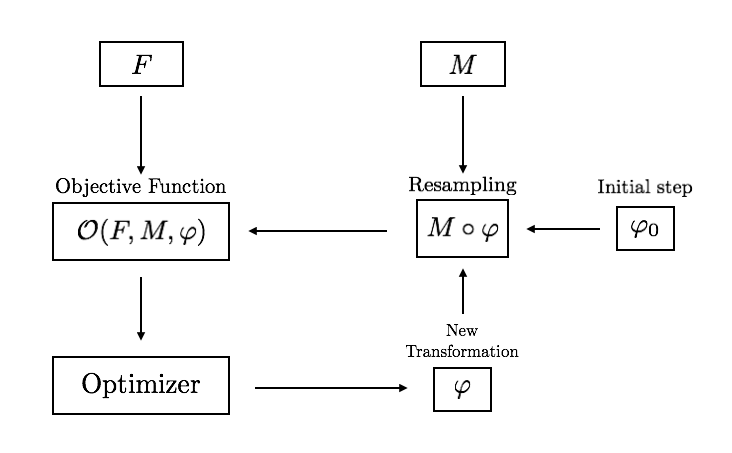
\includegraphics[scale=0.35]{figures/iterative_algorithm.png}
	\caption{Image registration framework scheme.}
	\label{fig:iterative_algorithm_scheme}
\end{figure}

\noindent
Just from this simplified scheme we can see that at each step moving and fixed images are defined within their domain, not necessarily coincident. 
It is always possible to define a common domain $\Omega = \Omega_{R}$, called  \emph{background space}, on which both of the images are defined.
%Avoid the resampling at each iteration decreases computational time, reduces artifacts and enable to have more control on the consequence of the chosen resampling technique.
%
%\begin{figure}[!ht]
%	\centering
%	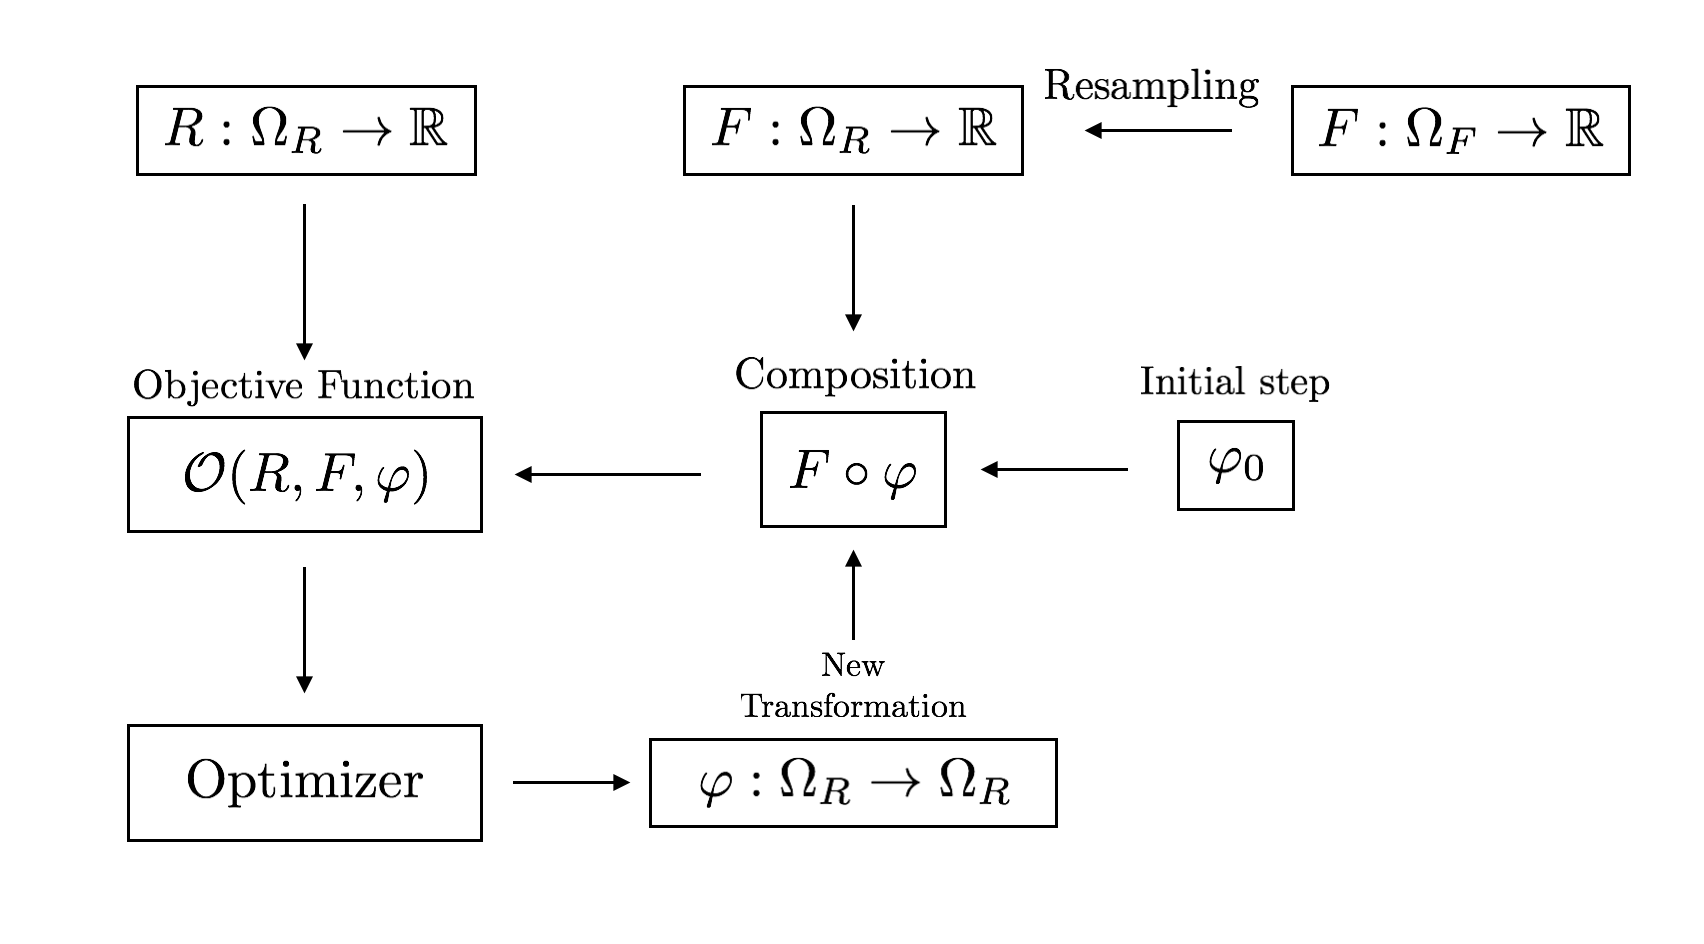
\includegraphics[scale=0.35]{figures/iterative_algorithm_res.png}
%	\caption{Image registration framework scheme.}
%	\label{fig:iterative_algorithm_scheme_modified}
%\end{figure}
\noindent
Far from being a complete overview of all of the possible framework does not take into account the fact that each version or implementation inevitably involves different needs and consequent challenges. Solutions found for each case may fall outside this simplification scheme: for example the parametrization of the transformations (or the deformation field's update) at each iterative step do not appear in this picture, even though is a fundamental feature. \\
In the following section we will going from the generalized framework to some specific aspects: we are interested in performing numerical computation to compute diffeomorphisms (bijective differentiable maps with differentiable inverse\footnote{Take the real valued $f(x)=x^3$: is bijective differentiable but the inverse is not everywhere differentiable.}). They are particularly appealing in medical imaging since in many situation biological modification do not involve any change in tissues' topology. We will see some details of parametrization of diffeomorphisms in five different frameworks: the LDDMM, the Shooting LDDMM, the Stationary LDDMM (or SVF), the DARTEL and the Demon.  In addition some details about the implementation of the image registration toolbox NiftyReg, used for some experiments in this research, can be found in the appendix.\\
Recent surveys in image registration can be found in \cite{Sotiras:survey:13} and \cite{Hill:survey:01}.

% % % % % % % % % % % % % % % % % % % % % % % % % % % % % % % % % % % % % %
% %  SECTION
% % % % % % % % % % % % % % % % % % % % % % % % % % % % % % % % % % % % % %
\section{Using Diffeomorphisms: Utility and Liability}

Idea of using diffeomorphisms can originate from two different perspective: if we imagine motion of captured images as motion of a fluid, we will start to approach the model using fluid dynamics; if we image motion as optical flow we will rely on differential geometry. Remarkably medical imaging application reveals common aspects of both underpinning theories, and requires some more since the discrete nature of actual input and output.\\
If we consider the rigid body transformation from classical mechanics, our transformations will be elements in $SE(3)$, the Lie group defined by combination of spatial rotations and translations. Five degrees of freedom, he possesses are enough to align 3d images; for continuous motions that maintains anatomical features between images they are not. We consider the Lie group of diffeomorphism $\text{Diff}(\Omega)$.
As already said, these functions are particularly appealing in computational anatomy since their topology-preserving nature, but their mathematical formalization has encountered many issues.\\ 
Attempt to provide this object some handle to manipulate it easily was done for the first time in 1966 in \cite{arnold1966geometrie}: to solve differential equation in hydrodynamic  $\text{Diff}(M)$ is considered as a Lie group with its Lie algebra. This assumption is not formally prosecuted in accordance to the problem-oriented nature of this paper\footnote{Subsequent steps in the exploration of the set of diffeomorphisms as a Lie group are \cite{marsden1970hamiltonian} and \cite{leslie1983lie}, \cite{omori1970group}. A survey on early development of infinite dimensional Lie group can be found in \cite{milnor1984remarks}.}.
The initial idea to consider $\text{Diff}(M)$ as a differentiable manifold involves to have it locally in correspondence with some generalized \lq\lq infinite-dimensional euclidean \rq\rq space. Attempt to set this correspondence showed that for some infinite-dimensional group the transition functions are smooth over Banach spaces. This led to the idea of Banach Manifolds. Unfortunately the group of diffeomorphisms do not belongs to the category of Banach manifold but requires a more generals space on which the transition map are smooth: the Frechet spaces. 
Thus the approach to the mathematical formalization of the general infinite dimensional Lie group involves Frechet differentiable manifolds. In this space we do not have anymore important theorems from analysis, as the inverse function theorem, or the main results from the Lie group theory in a finite dimensional settings, as Lie correspondence theorems.\\
These difficulties led some researcher in approaching the set of diffeomorphisms from other perspectives: for example, instead of treating $\text{Diff}(M)$ as group equipped with differential structures it is seen as a quotient of other well behaved group \cite{wojtynski1994one}.\\
Without denying the importance of fundamentals and underestimating the doors research in this domain may open, we will approach the matter in as similar way of what has been done in set theory: we will use a naive approach to infinite dimensional lie group, where the fundamental definition of infinite dimensional Lie group is a generalization of the finite dimensional case left to the intuition. 
We work then mostly on finite dimensional settings, relying on important theorems and easy close formulas, and we will extend methods and results developed here in the infinite case -clearly - with proper precautions.

%Besides, our purpose is not 'generalize definitions and theorems, while dodging counterexamples, but rather use the transformation groups for practical applications.


% % % % % % % % % % % % % % % % % % % % % % % % % % % % % % % % % % % % % %
% % SUB SECTION
% % % % % % % % % % % % % % % % % % % % % % % % % % % % % % % % % % % % % %
\subsection{LDDMM}

LDDMM \cite{beg2005computing} framework originates by considering motion between images as the motion of a fluid, and borrows its analytic tools from fluid dynamics. In this context the full set of homeomorphisms $\text{Hom}(\Omega)$ (continuous function from the background space $\Omega$ to itself with continuous inverse) is considered as a group with the composition. This group act\footnote{In this action it is preferable to consider the composition with the inverse, because this same action in differential geometry, called pull-back play the role of the contravariant operator of the push-forward, widely used to make a vector field act on a domain different from the one has been originally defined.} on the set of images defined on the background space $\mathcal{I}_{\Omega}$ as
\begin{align*}
\text{Hom}(\Omega) \times \mathcal{I}_{\Omega} & \longrightarrow  \mathcal{I}_{\Omega}   \\
(\varphi,F) &\longmapsto F\circ \varphi^{-1}
\end{align*}
The orbits of the subgroup of diffeomorphisms $\mathbb{G}$ on the image $F$, defined as
\begin{align*}
\mathcal{O}_{\mathbb{G}}(F) = \{ F\circ \varphi^{-1} \mid \varphi \in \mathbb{G} \}
\end{align*}
consists on all the images having the same topology\footnote{The idea of having the same topology is an analytical consequence of the definition of diffeomoprhism. Separated domains remains separated, although if they gets close enough, let say that their distance is less than the size of a voxel for a significant region, then the discretization will not maintain analytical topology and could broke it anyway.} of $F$.\\
In consequence of this, the Similarity term will be the distance between the moving image and the fixed image in the same orbit:
 \begin{align*}
 \text{Sim}(F,M,\varphi) = \frac{1}{\sigma^2}\euclideanMetric{F(\varphi^{-1})  - M  }_{L^{2}}^{2}
 \end{align*}
To define the regularization term that provides the optimal $\varphi$ at each step, in LDDMM (and subsequent frameworks) is considered the norm of the velocity vector field tangent to the transformation. Limiting is length means limiting the speed of the transformation at each step.
We consider a generic time varying vector field (TVVF) as the continuously differentiable map 
\begin{align*}
v:[0,1] & \longrightarrow  \text{Vect}(\Omega)\\
t  &\longmapsto  v_{t}  : \Omega \longrightarrow   \mathbb{R}^{d} \\
& \qquad \quad \quad \mathbf{x} \longmapsto v_{t}(\mathbf{x} )
\end{align*}
where $\text{Vect}(\Omega)$ is the set of all of the vector field over $\Omega$. With this notation $v$ is a vector field that changes continuously over a time parameter defined between $0$  and $1$. Once initial conditions are given, at each TVVF, corresponds a time varying homomorphisms defined  by the following ODE 
\begin{align}\label{eq:ode_phi_v}
\frac{d\phi_{t} (\mathbf{x})}{dt} = v_{t}(\phi_{t}(\mathbf{x} ))
\end{align}
where 
\begin{align*}
\phi : [0,1] & \longrightarrow  \text{Hom}(\Omega)\\
t  &\longmapsto \phi_{t}  : \Omega \longrightarrow    \Omega \\
& \qquad \quad \quad  \mathbf{x} \longmapsto \phi_{t}  (\mathbf{x} )
\end{align*}
Now the transformation $\varphi$ between fixed and moving images ($ R\circ \varphi^{-1} = T $) in which we where originally interested, can be defined within the couple $(v_{t},\phi_{t})$.  For $t = 0$, $\phi_{t} = Id$, identity of the group of homeomorphisms, and for $t = 1$, $\phi_{t} = \varphi$:
\begin{align*}
\varphi = \phi_{1} = \phi_{0} + \int_0^1 v_{t} (\phi) dt
\end{align*}
The set $\{ v_{t} (\phi) \mid t \in \lbrack 0,1 \rbrack \}$ is a path of transformations that varies continuously over the parameter $t$, starting at the identity and ending in the one the registration framework is looking for.\\
To have an efficient algorithm and a meaningful constraint on the resulting transformation, it is reasonable to consider $\phi_{t}$ as the shortest path between the identity and $\varphi$, so to have $v_{t} $ as the one that makes minimal the distance between transformations\footnote{This next equation can provide a metric on the manifold of the transformations, making it a Riemannian manifold. On the other side starting with a metric previously defined on the manifold, the consequence existence of geodesics may avoid the computation of the inf. In both cases this \lq\lq Riemannian approach\rq\rq  makes unavoidable the passage toward a metric, and makes the LDDMM a metric based algorithm.}:
\begin{align*}
l = \inf_{v_{t} ~ : ~ \dot{\phi_{t}} (\mathbf{x}) = v_{t}(\mathbf{x} )}  \int_{0}^{1} \euclideanMetric{v_{t}}_{L^2}^{2}dt
\end{align*}
In the LDDMM, ending points of path on the set of diffeomorphisms, whose tangent vector field (that varies over time) and can be used as regularization term:
\begin{align*}
\text{Reg}(F,M,\varphi) =  \int_0^1  \euclideanMetric{L v_{t} }_{L^{2}}^{2}  dt
\qquad 
\dot{\phi_{t}} (\mathbf{x}) = v_{t}(\mathbf{x} ) 
\quad 
\phi_{0} = Id
\quad 
\phi_{1} = \varphi
\end{align*}
Were $\varphi$ in the registration framework is the one provided by the optimization algorithm at the previous step, and $L$ is a linear operator that can be dependent on some parameters that makes the approach even more general\footnote{Recent approaches more image-oriented, proposed to use a kernel instead of an Operator.}. The operator $L$ is defined as $L = (\alpha\nabla + \gamma)$ for $\alpha$ and $\gamma$ real parameters and $\nabla$ the Laplace operator.\\
From the differential equation \ref{eq:ode_phi_v}, and in consequence of the definition of $\varphi$ the optimization function \ref{eq:general_cost_function} is defined as:
\begin{align*}
 \argmin_{v_{t} ~ : ~ \dot{\phi_{t}} (\mathbf{x}) = v_{t}(\mathbf{x} ) } 
\mathcal{O}(F, M, \varphi) 
= 
\argmin_{v_{t} ~ : ~ \dot{\phi_{t}} (\mathbf{x}) = v_{t}(\mathbf{x} ) } 
\int_0^1 \euclideanMetric{L v_{t} }_{L^{2}}^{2} dt + \frac{1}{\sigma^2}\euclideanMetric{F(\varphi^{-1})  - M  }_{L^{2}}^{2}
\end{align*}
And so the optimizer, at each step of the registration will look for
\begin{align*}
\hat{v} 
= 
\argmin_{v_{t} ~ : ~ \dot{\phi_{t}} (\mathbf{x}) = v_{t}(\mathbf{x} ) } 
\int_0^1 \euclideanMetric{L v_{t} }_{L^{2}}^{2} dt + \frac{1}{\sigma^2}\euclideanMetric{F(\varphi^{-1})  - M  }_{L^{2}}^{2}
\end{align*}
With this definition we see that is the $TVVF$, instead of the transformation $\varphi$, to be the output of the registration algorithm. On the computational side this appears even more natural in software implementation, the action of a diffeomorphisms $\varphi$ on an image is easily computed if the transformation is provided in term of discretized vector field $v_{t}$. \\
If $G$ is a cubic grid defined as the discretization of the background space $\Omega$, then a vector field dependent on time is parametrized as a 5-dimensional matrix
\begin{align*}
A = A(x,y,z,t,d) \qquad (x,y,z)\in G , ~~ t \in \lbrack 0,1\rbrack  ~~ d = 1,2,3
\end{align*}
where $(x,y,z)$ are discrete position of the grid, $t$ is the time parameter and $d$ is index of the coordinate axis. So the tangent vector $\mathbf{v}_{\tau}(x_0,y_0,z_0)$ at the point of the grid $(x_0,y_0,z_0)$, at time $\tau$, has Cartesian coordinate
\begin{align*}
\mathbf{v}_{\tau}(x_0,y_0,z_0) = (A(x_0,y_0,z_0,\tau,1), A(x_0,y_0,z_0,t,2), A(x_0,y_0,z_0,\tau,3))
\end{align*}
In the LDDMM approach, each transformation, in particular input and output of the optimization algorithm are discretized time varying velocity fields; the update at each step is given by
\begin{align*}
\mathbf{v}^{k+1} = \mathbf{v}^{k} - \epsilon \nabla d\mathcal{O}
\end{align*}
where $\mathbf{v}^{k}$ is the $k$-th step of the approximation, $d\mathcal{O}$ is the discretized version of the optimization function and $\epsilon$ is the gradient descent step size.
Details of the algorithms are provided in \cite{beg2005computing}; for purpose of this thesis it is important to notice that diffeomorphisms are used for the underpinning theory, as the solution of the differential equation \ref{eq:ode_phi_v}, and they are considered in the implementation while computing the similarity function; they are not used to compute the update at each step.

% % % % % % % % % % % % % % % % % % % % % % % % % % % % % % % % % % % % % %
% % SUB SECTION
% % % % % % % % % % % % % % % % % % % % % % % % % % % % % % % % % % % % % %
\subsection{Shooting LDDMM}

A direct upgrade of the 

Euler poincare equation to compute the momentum equation.


Only geodesics with initial condition.


\cite{vialard2012diffeomorphic}




% % % % % % % % % % % % % % % % % % % % % % % % % % % % % % % % % % % % % %
% % SUB SECTION
% % % % % % % % % % % % % % % % % % % % % % % % % % % % % % % % % % % % % %
\subsection{Stationary Velocity Fields LDDMM}



The approach of using time varying velocity field (TVVF) is a consequence of the differential equation involved in the registration problem. Solutions to differential equation depends on time. Another approach, is to start from the manifold structure on which the solution lives, the integral domain. In this context higher terms of differential equations are element of the tangent bundle. These objects do not originates from any differential equation, and retain their dignity of vector field even if independent form time parameters. The first time the passage form TVVF as solution to differential equation, to SVF as elements living in the tangent bundle of the integral domain of differential equation was done in \cite{arsigny2006log}. Using SVF in image registration algorithms have many advantages: a greedy strategy is adopted, so that at each iteration an update only of the stationary velocity field is computed and added to the one of the previous step. This makes the algorithm faster and less memory consuming. On the other side we have two main drawback: the possibility to perform statistics on SVF become less straightforward and the set of SFV is a subset of the diffeomorphisms with no group structure. More details on this will be seen in section \ref{se:svf_set}.

xxx parametrization of SVF

xxx the discretization

xxx the composition of SVF 

xxx how statistics can be performed relying on the tangent spaces


% % % % % % % % % % % % % % % % % % % % % % % % % % % % % % % % % % % % % %
% % SUB SECTION
% % % % % % % % % % % % % % % % % % % % % % % % % % % % % % % % % % % % % %
\subsection{DARTEL}


% % % % % % % % % % % % % % % % % % % % % % % % % % % % % % % % % % % % % %
% % SUB SECTION
% % % % % % % % % % % % % % % % % % % % % % % % % % % % % % % % % % % % % %
\subsection{Log-Demon}

In daemonology 

Dartel, LDDMM shooting, do not requires any log composition.
Log-composition is used in the 
1) Log-demon  - Tom
2) Bossa algorithm
3) Log euclidean by arsigny
4) Schild's Ladder - marco



In fact, given two TVVF $u_t$ and $v_t$ there is no straightforward operation that provides the TVVF that corresponds to the composition of the diffeomorphisms that generates these TVVF. To compute this, the vector field must be integrated to obtain the corresponding transformation $\psi$ and $\phi$. Corresponding transformation must be then composed and derived, to obtain again a TVVF that corresponds to the tangent vector field of the composition of $u_t$ and $v_t$.



% % % % % % % % % % % % % % % % % % % % % % % % % % % % % % % % % % % % % %
% % SECTION
% % % % % % % % % % % % % % % % % % % % % % % % % % % % % % % % % % % % % %
\section{Stationary Velocity Fields and the Composition of Diffeomorphisms in the Tangent Space}

% why do we need compositon of diffeomorphisms in diffeomorphic image registration. Why it is such a crucial thing and why it is difficult.
% Heay computations involved, lack of a close formula, and so on... The task is hard but we are brave enough to try!!

\noindent
xxx computational anatomy and the need for statistics.

\noindent
xxx introduction of log and exp concepts (formally later, in section \ref{se:lie_exp_log_comp} ).

\noindent
xxx starting from vectors, ending with one vector: the log composition, idea, not formally defined.

\noindent
defined as the vector $\mathbf{w}$ in the Lie algebra $\mathfrak{g}$ that reflects the composition in the Lie group of two vectors $\mathbf{u}, \mathbf{v}$ in the same tangent space:
\begin{align*}
\mathbf{w} = \log(\exp(\mathbf{u})\circ\exp( \mathbf{v}))
\qquad
\forall \mathbf{u}, \mathbf{v} \in \mathfrak{g}
\end{align*}


\noindent
xxx the BCH formula, as the first method to compute the log-composition.











%Under this light, the transitions from the Lie group to Lie algebra (the Lie logarithm) and its return (the Lie exponential) become fundamental tools.
%The main topic of this research is the evaluation of the operation that we define here as \emph{Lie algebra Group Composition}, or simply \emph{Group Composition}, 
%
%
%
%
%One of the Matrix Lie group explored in this research is the special euclidean group $\text{SE}(d)$, or group of rigid transformations.
%A little increase in the number of degrees of freedom leads to the group of the affine transformations, where scaling and shearing have been added to the possible transformations. \\
%The idea of maximize the number of degrees of freedom in a transformation that maintains anatomical features between images, led to consider the Lie group of diffeomorphism $\text{Diff}$.
%A diffeomorphism $p$ can be expressed as the sum of the identity function with a differentiable transformation depending on $\mathbf{x}$. It is possible to write:
%\begin{align*}
%p(\mathbf{x})  = \mathbf{x} + \gamma(\mathbf{x})
%\end{align*}
%With this notation the vector $\dot{\gamma}(\mathbf{x})$ is the speed\footnote{as we will see, a feasible way to express a set of diffeomorphisms is as the solution of the differential equation defined by the velocities of the transformation.} of each point from its original to a new position due to the application of $p$.\\
%In the iterative diffeomorphic registration algorithm (in which the structure is defined by regularization and similarity), to obtain the update at each step, it is required to apply consecutively two diffeomorphisms $p_{i}$ and  $\hat{p}_{i+1}$ and consider the resulting composition as the required update.
%%\begin{figure}[!ht]
%%	\centering
%%	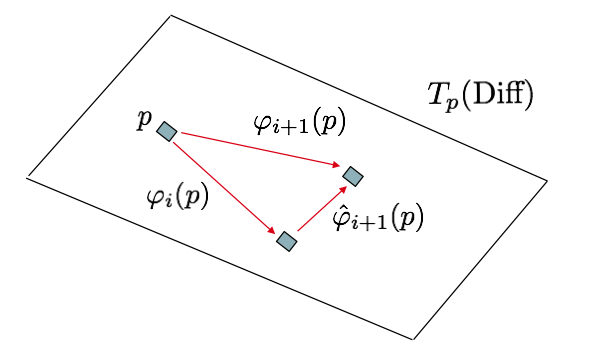
\includegraphics[scale=0.35]{figures/diff_update.png}
%%	\caption{Composition of tangent vectors of diffeomorphism (provisional).}
%%	\label{fig:composition1}
%%\end{figure}
%As a consequence, the corresponding vector of the transformation $p_{i+1}$ in the tangent space of the Lie group can be computed, given two vectors in the tangent bundle, with an operation called here \emph{the group composition in the Lie algebra}.\\
%In \cite{Bossa2007} the BCH formula appears as an improvement of the scaling and squaring algorithm to compute the logarithm of a matrix. As noticed in the same paper, the BCH formula is used in a infinite dimensional settings, while its validity has been proven only for finite dimensional Lie group. In addition while composing the logarithm of a composition of two exponentials, the initial tangent vectors belongs to the same tangent space. This is not the case while composing $p_{i}$ with $\hat{p}_{i+1}$ the tangent vector that defines $\hat{p}_{i+1}$ is an element of the tangent plane to $p_{i}$. \\
%Is it possible to reach a proper computation thanks to the definition of Affine exponential, that differs from the Lie exponential used in \cite{Bossa2007} .
%
%
%
%
%
%
%The BCH formula provides an expression of the Group Composition in the finite dimensional case expressed as an infinite series of nesting commutators. The difficulties involved in dealing with this formula, as well as its non completely proper use in the infinite dimensional setting, gave birth to some methodologies and approaches, whose investigation is the main goal of this research. One of these approaches, involves the Taylor expansion and has a computable form in the finite dimensional. A geometrical approach that holds also in the infinite dimensional case is the parallel transport.
%It can be considered as a natural approach to evaluate the group composition with offset. It consists in the transport of the vector $\mathbf{v}$ along the geodesic having $\mathbf{u}$ as tangent vector such that during the transport it maintains the condition of parallelism. The resulting vector $\mathbf{v}^{\parallel}$ in the tangent plane of $\mathbf{u}$ can be then summed with $\mathbf{v}$ with similar results to the direct application of the BCH. Its evaluation involves the Schild's ladder and the pole ladder. Both have already found practical application in medical imaging \cite{Lorenzi:discrete_ladders:14}, \cite{Lorenzi:pt:13}.
%Parallel transport is necessarily related with the definition of the connection. Choosing among possible connections become a crucial feature, whose consequences in the corresponding realization in the transformation of images requires further studies.
%
%\begin{figure}[!ht]
%	\centering
%	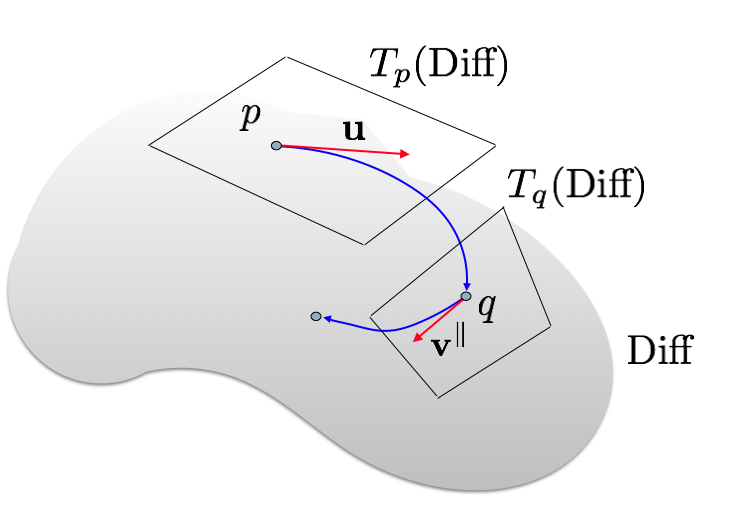
\includegraphics[scale=0.25]{figures/parallel_transport_1.png}
%	\caption{Group composition with offset using parallel transport.}
%	\label{fig:composition}
%\end{figure}
%
%The lack of a close form of any kind and the theoretical difficulties inherent to the investigation of infinite dimensional group of diffeomorphism makes an experimental approach meaningful. 











